\apendice{Especificación de Requisitos}
Este apéndice se subdivide en los diferentes requisitos necesarios para nuestro proyecto, en su realización y subdivisión. 
\section{Objetivos Generales}
\begin{enumerate}
\item Construir un cuestionario anónimo para la recogida de datos iniciales para ser utilizados en el entrenamiento de los sistemas de recomendación. 
\item Desarrollar  diferentes sistemas de recomendación, su entrenamiento en base a los datos recogidos y la devolución de las ponderaciones de las asignaturas no cursadas por un usuario. 
\item Desarrollar una interfaz gráfica modo usuario para una mejor utilización de los mismos, de forma que las recomendaciones mostradas por el sistema de recomendación sean específicas para determinado usuario. 
\item Desarrollar de una interfaz gráfica modo administrador para la modificación, agregación o eliminación de diferentes calificaciones. 
\end{enumerate}
\section{Catálogo de Requisitos}
\begin{itemize}
\item RF-1. Recogida de datos\\ 
\begin{itemize}
\item RF-1.1. Creación de cuestionario anónimo.\\ 
\item RF-1.2. Distribución del cuestionario. \\ 
\item RF-1.3. Recogida de datos y su almacenamiento. 
\end{itemize}

\item RF-2. Desarrollo de los sistemas de recomendación\\ 
\begin{itemize}
\item RF-2.1. Recogida de datos de Drive, Fichero Biario y/o Base de Datos. 
\item RF-2.2. Tratamiento de los datos. 
\item RF-2.3. Desarrollo del sistema de recomendación. 
\item RF-2.4. Devolución de las calificaciones. 
\item RF-2.5. Guardado de los datos. 
\end{itemize}

\item RF-3. Desarrollo de una interfaz gráfica \\ 
\begin{itemize}
\item RF-3.1. Construcción de pestaña de inicio sesión.  
\item RF-3.2.Lectura de datos almacenados. 
\item RF-3.3 Obtención de datos del registro de usuario. 
\item RF-3.4.Generación de recomendación de calificaciones. 
\item RF-3.5.Muestra de gráficos de calificaciones en diferentes asignaturas. 
\item RF-3.6.Muestra de gráficos auxiliares para mayor información al usuario. 
\item RF-3.7.Acceso a los datos generales en modo administrador. 
\end{itemize}

\end{itemize}

\section{Especificación de Requisitos}
\begin{itemize}


\item Construcción de ventana de inicio de sesión. 
\begin{itemize}
\item Construcción de botón de inicio sesión. 
\item Construcción de áreas para rellenar usuario y contraseña.  
\item Construcción de la funcionalidad para acceder a la Base de Datos. 
\item Construcción de la funcionalidad para validar usuario y contraseña. 
\end{itemize}

\item Construcción de la funcionalidad de la recogida,  guardado y  el tratamiento de los datos. 
\begin{itemize}
\item Construcción de la funcionalidad de recogida de datos de Drive. 
\item Construcción de la funcionalidad del tratamiento de los datos recogidos. 
\item Construcción de la funcionalidad para el guardado de los datos. 

\end{itemize}

\item Construcción de la pestaña inicial para rellenar el cuestionario para ponderar las asignaturas cursadas. 
\begin{itemize}
\item Construcción de la funcionalidad de los botones para seleccionar los cursos para ponderar sus asignaturas. 
\item Construcción de la funcionalidad para guardar en local los resultados introducidos. 
\item Construcción de la funcionalidad para poder modificar las ponderaciones introducidas. 
\item Construcción de la funcionalidad para seleccionar una asignatura como no aplicada. 
\item Construcción de la funcionalidad para no contabilizar dicha asignatura en el sistema de recomendación. 
\item Construcción de la funcionalidad para cargar los datos desde Base de Datos. 
\item Construcción de la funcionalidad para almacenar los datos en la Base de Datos. 
\end{itemize}

\item Construcción de las pestañas para la recomendación de las asignaturas. 
\begin{itemize}
\item Construcción de los botones  de selección del Sistema de Recomendación.
\item Construcción de funcionalidad para llamar al sistema de recomendación  seleccionado. 
\item Construcción de la funcionalidad para ejecutar el sistema de recomendación con los datos rellenados. 
\item Construcción de la funcionalidad para mostrar las calificaciones resultantes no cursadas. 
\item Construcción de la funcionalidad para mostrar gráficos de dicha recomendación. 
\end{itemize}

\item Construcción de la pestaña para la muestra de gráficos auxiliares. 
\begin{itemize}
\item Construcción de la funcionalidad para mostrar la media aritmética del curso. 
\item Construcción de la funcionalidad para mostrar gráficos auxiliares de las preferencias de las asignaturas. 
\end{itemize}

\end{itemize}

\section{Diagramas de Casos de Uso}
\subsection{Diagrama General}
El siguiente diagrama corresponde al  caso de uso general, junto con el diagrama extendido. ~\ref{fig:Diagrama_Caso_Uso_General}
\begin{figure}[h]
\centering
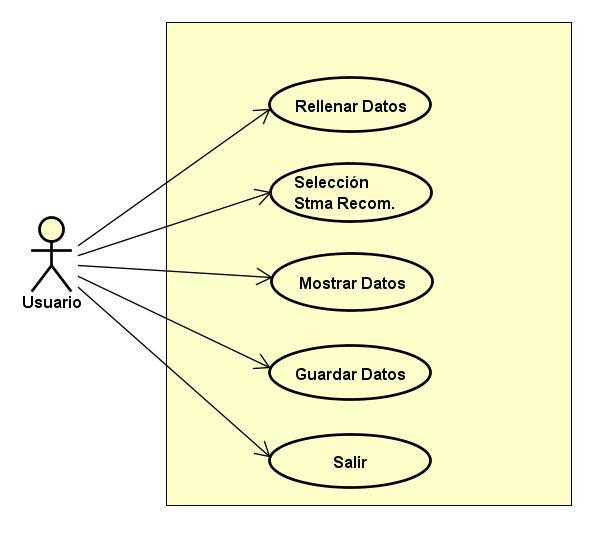
\includegraphics[width=0.90\textwidth]{Diagrama_Caso_Uso_General}
\caption{Diagrama de caso de uso General}
\label{fig:Diagrama_Caso_Uso_General}
\end{figure}

\section{Tablas de Casos de Uso Generales}
\subsection{Primer Caso de Uso}
La primera tabla corresponde al desarrollo del cuestionario anónimo y la recogida de datos para poder trabajar posteriormente con ellos. La siguiente tabla hace referencia al dicho caso de uso. \ref{tab:1}
\begin{table}[]
\caption{Tabla Caso de Uso 1}
\label{tab:1}
\resizebox{\textwidth}{!}{
\begin{tabular}{ lrrr }
\toprule
\textbf{Nombre} &   Recogida de Datos         \\ 
\textbf{Versión} & 1.0  \\ 
\textbf{Requisitos Funcionales}  & \begin{tabular}[c]{@{}l@{}}RF-1\\ RF-1.1\\ RF-1.2\\ RF-1.3\\\end{tabular}                                                                                                                  \\ 
\textbf{Descripción de Requisitos} & \begin{tabular}[r]{@{}l@{}}Se obtendrán los datos de forma anónima  para el entrenamiento\\ de los sistemas de recomendación\\\end{tabular}                                                                                                                    \\
\textbf{Precondiciones}     &Conexión a Internet. \\
\textbf{Postcondiciones}         &  Se almacenarán los datos en una API de Google \\
\textbf{Autor}         & Clara Palacios Rodrigo \\
\textbf{Importancia}        &  Importante \\ \bottomrule
\end{tabular}
}
\end{table}

\subsection{Segundo Caso de Uso}
La segunda tabla corresponde con el desarrollo de los sistemas de recomendación. Para ello, se debe obtener los datos de la API de Drive, tratarlos y desarrollar los diferentes sistemas de recomendación. La siguiente tabla hace referencia a dicho caso de uso. ~\ref{tab:2}
\begin{table}[]
\caption{Tabla Caso de Uso 2}
\label{tab:2}
\resizebox{\textwidth}{!}{
\begin{tabular}{ lrrr }
\toprule
\textbf{Nombre} &   Desarrollo de los sistemas de recomendación        \\ 
\textbf{Versión} & 1.0  \\ 
\textbf{Requisitos Funcionales}  & \begin{tabular}[c]{@{}l@{}}RF-2\\ RF-2.1\\ RF-2.2\\ RF-2.3\\RF-2.4\\RF-2.5\end{tabular}                                                                                                                  \\ 
\textbf{Descripción de Requisitos} & \begin{tabular}[c]{@{}l@{}}Se permitirá el acceso a los datos globales para el sistema de recomendación\\  así como la obtención de los mismos.\\\end{tabular}                                                                                                                     \\
\textbf{Precondiciones}     & \begin{tabular}[c]{@{}l@{}} Disponer de los datos en Drive\\ Disponer de los Sistemas de Recomendación\\\end{tabular}                                                                                                                   \\
\textbf{Postcondiciones}         &  Devolución de los resultados \\
\textbf{Autor}         & Clara Palacios Rodrigo \\
\textbf{Importancia}        & Muy Importante \\ \bottomrule
\end{tabular}
}
\end{table}


\subsection{Tercer Caso de Uso}
La tercera tabla corresponde con  el desarrollo de la interfaz gráfica, así como la funcionalidad de los botones de la misma. De esta forma, se mostrarán los datos en la interfaz de acuerdo con el entrenamiento de los sistemas de recomendación con los datos introducidos por el usuario, así como gráficos correspondientes a dichos datos y a los resultados obtenidos por el sistema de recomendación seleccionado. La siguiente tabla hace referencia a dicho caso de uso. ~\ref{tab:3}
\begin{table}[]
\caption{Tabla Caso de Uso 3}
\label{tab:3 }
\resizebox{\textwidth}{!}{
\begin{tabular}{ lrrr }
\toprule
\textbf{Nombre} &  Desarrollo de una interfaz gráfica  \\ 
\textbf{Versión} & 1.0  \\ 
\textbf{Requisitos Funcionales}  & \begin{tabular}[c]{@{}l@{}}RF-3\\ RF-3.1\\ RF-3.2\\ RF-3.3\\RF-3.4\\RF-3.6\\RF-3.7\end{tabular}                                                                                                                  \\ 
\textbf{Descripción de Requisitos} & \begin{tabular}[c]{@{}l@{}}Se recogerán los datos al usuario y se mostrarán gráficos y resultados\\obtenidos del sistema de recomendación escogido.\\\end{tabular}                                                                                                                     \\
\textbf{Precondiciones}     & \begin{tabular}[c]{@{}l@{}}Disponer de una interfaz gráfica.\\Haber solicitado los datos al usuario\\Tener al usuario registrado en la BD.\end{tabular}                                                                                                                     \\
\textbf{Postcondiciones}         &  Devolver correctamente las calificaciones. \\
\textbf{Autor}         & Clara Palacios Rodrigo \\
\textbf{Importancia}        & Muy Importante \\ \bottomrule
\end{tabular}
}
\end{table}


\section{Requisitos necesarios}
Esta sección consistirá en el desarrollo de los requisitos funcionales de forma detallada explicando sus pasos a seguir, así como qué es necesario para cada requisito. 
\subsection{RF-1}
La recogida de datos se ha realizado modo online. Se ha distribuido entre los alumnos del cuarto curso y antiguos alumnos de la carrera. 
\subsubsection{RF-1.1}
Creación de un cuestionario anónimo. Para este requisito funcional se ha requerido: 
\begin{itemize}
\item Conexión  y acceso a Internet. 
\item Registro en la página de Typeform. 
\item Conocimiento de las asignaturas existentes en el Grado de Ingeniería Informática. 
\item Creación de un cuestionario anónimo de ponderaciones. 
\item Selección del modo de guardado de los datos recabados. 
\end{itemize}

\subsubsection{RF-1.2}
Para la distribución del cuestionario anónimo entre los diferentes alumnos, se ha solicitado ayuda a: 
\begin{itemize}
\item Tutor José Ignacio Santos Martín. 
\item Javier López Martínez para la distribución mediante un correo en la Asociación de Ingenieros Informáticos. 
\item Delegado del cuarto curso. 
\end{itemize}

\subsubsection{RF-1.3}
Para la recogida y el almacenamiento de datos, se ha utilizado el API de Google Drive, en donde se almacenan los datos con un refresco de 3 minutos en una tabla de Excel. Para ello, se debe disponer de: 
\begin{itemize}
\item Conexión a Internet para el acceso a los datos. 
\item Disponer de una cuenta Gmail. 
\item Tener habilitado el API de Google Drive. 
\end{itemize}

\subsection{RF-2}
Para el desarrollo de los sistemas  de recomendación se debe haber obtenido los datos del cuestionario anónimo de forma previa. 
\subsubsection{RF-2.1}
Para el acceso a los datos, bien  desde fichero binario almacenado en local, bien desde la API de GoogleDrive, bien desde Base de Datos en Cloud, se requiere: 
\begin{itemize}
\item Acceso a los datos en Drive, haciendo uso del API GoogleDrive y el fichero json obtenido de forma previa. 
\item En caso de disponer de conexión a Internet, se accederá a la base de datos en Cloud, en caso contrario, se debe tener una base de datos en local para el acceso de los mismos. Para ello, se debe disponer de ambas bases de datos, en donde residan  los datos recabados. 
\end{itemize}

\subsubsection{RF-2.2}
Los datos, bien obtenidos de fichero binario, bien de la base de datos o bien de GoogleDrive, deben ser tratados para ser devueltos como un DataFrame. En este aspecto, se debe tener en cuenta: 
\begin{itemize}
\item Acceso a Internet en caso de que los datos se encuentren en la API de GoogleDrive. 
\item Conocimiento del lenguaje de programación para tratar los datos de la forma más óptima posible. 
\item Eliminación de las columnas innecesarias recabadas. 
\item Sustitución de las columnas vacías por NaN. 
\item Devolución de un Dataframe estructurado. 
\end{itemize}

\subsubsection{RF-2.3}
Se deben implementar los sistemas de recomendación deseados. Para ello, es necesario: 
\begin{itemize}
\item Conocimiento de la implementación de los sistemas de recomendación. 
\item Disponer de los datos para el entrenamiento de los sistemas de recomendación. 
\item Desarrollo de los sistemas de recomendación.
\end{itemize}


\subsubsection{RF-2.4}
Una vez ejecutado el sistema de recomendación, éste debe devolver   las calificaciones de las asignaturas de Cuarto no cursadas. Por ello: 
\begin{itemize}
\item Se debe devolver las asignaturas no cursadas ordenadas de mayor a menor. 
\item Junto con los nombres de las asignaturas, se deben devolver las calificaciones obtenidas. 
\end{itemize}

\subsubsection{RF-2.5}
Tras obtener las calificaciones de las asignaturas se deben guardar bien en la base de datos o bien en un fichero binario, para acceder a ellos posteriormente. 
\begin{itemize}
\item Se debe disponer de una base de datos o un fichero binario. 
\item Se debe tener conocimiento de Bases de datos y ORM.  
\end{itemize}


\subsection{RF-3}
El tercer requisito funcional hace referencia a la interfaz gráfica, su desarrollo e implementación. 
\subsubsection{RF-3.1}
Para la construcción de la pestaña de inicio sesión debe existir una base de datos de forma previa, bien en local o en Cloud, para poder validar el usuario y contraseña. Por otra parte, para el cumplimiento de la LOPD, tanto los datos íntegros del usuario deben permanecer seguros. 
\begin{itemize}
\item Lectura de usuario y contraseña. 
\item Acceso a la Base de Datos. 
\item Encriptación de la contraseña. 
\item Corroborar usuario y contraseña con la BD. 
\item Devolución de una respuesta aceptando o rechazando la conexión. 
\end{itemize} 

\subsubsection{RF-3.2}
Tras iniciar sesión, en caso de existir el usuario, se deben leer los datos almacenados del usuario y las calificaciones que haya realizado a las diferentes asignaturas. 
\begin{itemize}
\item Lectura de las calificaciones de dicho usuario. 
\item Devolución de las calificaciones. 
\item Recepción de las calificaciones. 
\item Muestra  de las calificaciones en la pestaña de asignaturas. 
\end{itemize} 

\subsubsection{RF-3.3}
En caso de registrarse el usuario, se debe solicitar sus datos y almacenarlos en la base de datos de forma segura, además de solicitarle rellenar las calificaciones de las asignaturas. 
\begin{itemize}
\item Lectura de los datos introducidos por el usuario. 
\item Almacenamiento de los datos del usuario en la BD.  
\item Lectura de las calificaciones de dicho usuario. 
\item Almacenamiento de las calificaciones.  
\end{itemize} 

\subsubsection{RF-3.4}
Tras obtener los datos de la BD, se deben almacenar para los cálculos del sistema de recomendación (RF-2.3  y RF-2.4) y mostrarlos por pantalla de forma ordenada. 
\begin{itemize}
\item Ejecutar los sistemas de recomendación con los datos obtenidos.  
\item Ordenación de las asignaturas por sus calificaciones. 
\item Muestra de las 10 asignaturas con la mayor ponderación. 
\item Almacenamiento de las calificaciones.  
\end{itemize} 


\subsubsection{RF-3.5}
En la pestaña de las recomendaciones, se debe mostrar unos gráficos de dichas asignaturas. Los datos utilizados son los obtenidos de los sistemas de recomendación. 
\begin{itemize}
\item Se deben tener las asignaturas con mayores calificaciones almacenadas. 
\item Mostrar de forma ordenada (sin redondear), en diagrama de barras las asignaturas. 
\item Mostrar un gráfico de los campos a los que pertenecen dichas asignaturas. 
\end{itemize} 

\subsubsection{RF-3.6}
En la tercera pestaña, se muestran medias de las ponderaciones de las asignaturas de los usuarios existentes en la BD, de forma que se puede observar, con una visión global, las preferencias generales de los alumnos. 
\begin{itemize}
\item Se debe acceder a los datos de los usuarios. 
\item Se deben calcular las medias con dichos usuarios. 
\item Separar las asignaturas por cursos. 
\item Mostrar las medias de las asignaturas por cursos en diagramas de barra. 
\end{itemize} 

\subsubsection{RF-3.7}
Se debe permitir, en modo administrador, acceder a los datos para poder añadir, modificar y eliminar las asignaturas. Hasta el momento, dicha interfaz no está implementada. 
\begin{itemize}
\item Se debe iniciar sesión obteniendo una interfaz diferente. 
\item Se debe acceder a la BD para la inclusión de nuevas asignaturas. 
\item Se deben permitir guardar dichos datos en la BD en Cloud. 

\end{itemize} 
